\NeedsTeXFormat{LaTeX2e}[2005/12/01]
%%    2009/03/12 v1.0 GAUBM Vorlage für Aschlussarbeiten Physik
%% Template fuer Bachelor- und Masterarbeiten
%% an der Fakultaet fuer Physik (c) Thomas Pruschke der GA Universität
%% Verbesserungsvorschlaege bitte an pruschke@theorie.physik.uni-goettingen.de
%%
%% Benoetigte Pakete: datenumber
%%

%%%%%%%%%%%%%%%%%%%%%%%%%%%%%%%%%%%%%%%%%%%%%%%%%%%%%%%%%%%%%%%%%%%%%%
%%%%%%%%%% Bitte vor dem Veraendern diese Datei umbenennen! %%%%%%%%%%
%%%%%%%%%%%%%%%%%%%%%%%%%%%%%%%%%%%%%%%%%%%%%%%%%%%%%%%%%%%%%%%%%%%%%%

%% scrbook - Ersatz für LaTeX book Klasse aus dem KOMA Script
%% Moegliche Optionen: diejenigen der Klasse scrbook ausser titlepage

%% deutsche Arbeit:
\documentclass[bachelor,       %% Typ der Arbeit: bachelor oder master
               twoside,        %% zweiseitiges Layout
               BCOR10mm,       %% Bindekorrektur 10 mm
%               liststotoc,nomtotoc,bibtotoc, %% Aufnahme der div. Verzeichnisse
                                              %% ins Inhaltsverzeichnis
               english,ngerman, %% Alternativspr. Englisch, Dokumentspr. Deutsch
%               ngerman,english  %% Alternativspr. Deutsch, Dokumentspr. Englisch
%               final,          %% Endversion; draft fuer schnelles Kompilieren
               ]{GAUBM}

\usepackage{setspace}  %% Zur Setzung des Zeilenabstandes
\usepackage{babel}     %% Sprachen-Unterstuetzung
\usepackage{calc}      %% ermoeglicht Rechnen mit Laengen und Zaehlern
\usepackage[T1]{fontenc}       %% Unterstutzung von Umlauten etc.
%\usepackage[latin1]{inputenc}  %% 
%% in aktuellem Linux & MacOS X wird standardmaessig UTF8 kodiert!
\usepackage[utf8]{inputenc}    %% Wenn latin1 nicht geht ...

\usepackage{amsmath,amssymb} %% zusaetzliche Mathe-Symbole

\usepackage{lmodern} %% type1-taugliche CM-Schrift als Variante zur
                     %% "normalen" EC-Schrift
%% Paket fuer bibtex-Datenbanken
%\usepackage[comma,numbers,sort&compress]{natbib}
\usepackage{babelbib}
\selectbiblanguage{ngerman}
\bibliographystyle{apalike}

\newcommand{\tabheadfont}[1]{\textbf{#1}} %% Tabellenkopf in Fett
\usepackage{booktabs}                      %% Befehle fuer besseres Tabellenlayout
\usepackage{longtable}                     %% umbrechbare Tabellen
\usepackage{array}                         %% zusaetzliche Spaltenoptionen

%% umfangreiche Pakete fuer Symbole wie \micro, \ohm, \degree, \celsius etc.
\usepackage{textcomp,gensymb}

%\usepackage{SIunits} %% Korrektes Setzen von Einheiten
\usepackage{units}   %% Variante fuer Einheiten

%% Hyperlinks im Dokument; muss als eines der letzten Pakete geladen werden
\usepackage[pdfstartview=FitH,      % Oeffnen mit fit width
            breaklinks=true,        % Umbrueche in Links, nur bei pdflatex default
            bookmarksopen=true,     % aufgeklappte Bookmarks
            bookmarksnumbered=true  % Kapitelnummerierung in bookmarks
            ]{hyperref}

%% Weiter benoetigte Pakete: datenumber
%% Falls dieses Paket nicht in der Installation vorhanden ist,
%% kann es von der Seite mit diesem Template heruntergeladen werden
%% und in einem LaTeX bekanntem Verzeichnis installiert werden (notfalls
%% dem Verzeichnis mit der Arbeit).

% Mehrere Abbildungen nebeneinander
\usepackage{subfigure}
\usepackage{adjustbox}

\begin{document}
%%
%%                   Ab hier muessen die Anpassungen geschehen
%%
%% Hier den eigenen Namen einsetzen
\ThesisAuthor{Felix}{Kurtz}
%% Hier den Geburtsort einsetzen
\PlaceOfBirth{Bad Nauheim}
%% Titel Arbeit. Das erste Argument ist der deutsche, das zweite der
%% englische Titel.
\ThesisTitle{Beobachtung von Doppelpulsen im KLM-Ti:Sa-Laser mittels Einzelschuss-Spektroskopie}{Observation of double pulses in a KLM-Ti:Sa Laser with single-shot spectroscopy}
%% Erst- und Zweitgutacher/in
%% Ist der/die Betreuer/in nicht identisch mit dem/r Erstgutachter/in,
%% muss diese/r als optionales Argument angegeben werden.
\FirstReferee[Dr.\ Georg Herink]{Prof.\ Dr.\ Claus Ropers}
\Institute{4.Physikalischen Institut}
\SecondReferee{Prof.\ Dr.\ Stefan Mathias}
%% Beginn und Ende des Anfertigungszeitraumes
\ThesisBegin{1}{4}{2016}
\ThesisEnd{15}{7}{2016}
%% DO NOT TOUCH THESE LINES!!!!
\frontmatter
\maketitle
\cleardoublepage
%% Zusammenfassung. Falls nicht gewuenscht, bitte auskommentieren.
\begin{abstract}
  Hier werden auf einer halben Seite die Kernaussagen der Arbeit
  zusammengefasst.
%% Optional: Stichwoerter. Wenn nicht gewuenscht, koennen die beiden
%% folgenden Zeilen geloescht werden
  \bigskip\par
  \textbf{Stichwörter:} Physik, Bachelorarbeit
\end{abstract}
%% So laesst sich in die andere Sprache umschalten (Englisch bzw. Deutsch)
\begin{otherlanguage}{english}
\begin{abstract}
  Here the key results of the thesis can be presented in about
  half a page.
  \bigskip\par
  \textbf{Keywords:} Physics, Bachelor thesis
\end{abstract}
\end{otherlanguage}

%% Ende des Vorspanns
\cleardoublepage
%% Ab hier 1 1/2 facher Zeilenabstand (durch setspace-Paket)
\onehalfspacing
%% Erzeugt Inhaltsverzeichnis
\tableofcontents

%%% Hier kann man seine Bezeichnungsweisen erklaeren. Falls nicht
%%% benoetigt, bis einschliesslich \end{nomenclature} auskommentieren
%\begin{nomenclature}
%%% Fuer die Berechnung der Spaltenbreiten muss \usepackage{calc}
%%% geladen sein!
%\section*{Lateinische Buchstaben}
%\noindent
%\begin{longtable}[l]{p{0.2\textwidth}p{0.7\textwidth-6\tabcolsep}p{0.1\textwidth}}
%  \tabheadfont{Variable}&\tabheadfont{Bedeutung}&\tabheadfont{Einheit}\\\midrule\endhead
%  $A$ & Querschnittsfl"ache & $\unit{m^2}$\\
%  $c$ & Geschwindigkeit & $\unitfrac{m}{s}$
%\end{longtable}
%\section*{Griechische Buchstaben}
%\begin{longtable}[l]{p{0.2\textwidth}p{0.7\textwidth-6\tabcolsep}p{0.1\textwidth}}
%  \tabheadfont{Variable}&\tabheadfont{Bedeutung}&\tabheadfont{Einheit}\\\midrule\endhead
%  $\alpha$  & Winkel & $\unit{\degree}$; --\\
%  $\varrho$ & Dichte & $\unitfrac{kg}{m^3}$
%\end{longtable}
%\section*{Indizes}
%\begin{longtable}[l]{p{0.2\textwidth}p{0.8\textwidth-4\tabcolsep}}
%  \tabheadfont{Index}&\tabheadfont{Bedeutung}\\\midrule\endhead
%  m & Meridian\\
%  $r$ & Radial
%\end{longtable}
%\section*{Abk"urzungen}
%\begin{longtable}[l]{p{0.2\textwidth}p{0.8\textwidth-4\tabcolsep}}
%  \tabheadfont{Abk"urzung}&\tabheadfont{Bedeutung}\\\midrule\endhead
%  2D & zweidimensional\\
%  3D & dreidimensional\\
%  max & maximal
%\end{longtable}
%\end{nomenclature}
%% \listoftables und \listoffigures sollten nur bei genuegender Anzahl Tabellen
%% verwendet werden
%\listoffigures
%\listoftables

\mainmatter   %% Anfang Hauptteil

\chapter{Einleitung}
Femtosekundenlaser sind heutzutage aus der aktuellen Forschung nicht mehr wegzudenken.
Besonders Titan-Saphir-Laser werden häufig eingesetzt, weil sie die kürzesten Pulse mit wenigen optischen Zyklen emittieren können.
Wenn diese richtig eingestellt sind, laufen sie auch ultrastabil und reproduzieren das immer gleiche Spektrum.
Anders sieht das allerdings aus, wenn man den Laser so justiert, dass nicht nur ein Puls im Laser umher läuft, sondern zwei oder mehrere.
Dann kann es zu Interaktionen zwischen den Pulsen kommen.
Dieses dynamische Verhalten konnte zuvor noch nicht in Echtzeit beobachtet werden.
Mit der hier genutzten Methode der \textit{dispersiven Fouriertransformation} ist es nun möglich, das Spektrum jedes einzelnen Pulses bzw. Pulspaares aufzunehmen und in letzterem Fall daraus den Abstand sowie die Phase zwischen den beiden Pulsen zu bestimmen.
Dies eröffnet ganz neue Einblicke in die Welt der Laserdynamik.


\chapter{Grundlagen}

\section{Der Laser}
Der zu untersuchende Laser ist ein Titan:Saphir-Laser (\textit{Rainbow} von \textit{FemtoLasers}).
Er erzeugt 7-fs-Pulse bei einer Puls-Wiederholrate von $80\,$MHz und einer Leistung von mehr als $250\,$mW.
\subsection{Mode-Locking}
Damit der Laser solche kurzen Pulse erzeugen kann, müssen viele Longitudinal-Moden in der Cavity in Phase sein.
Dieses \emph{Mode-Locking} wird dadurch erreicht, dass hohe Intensitäten im Laser nichtlinear verstärkt werden.
Hier wird das durch den \textbf{Kerr-Effekt} erreicht, also den intensitätsabhängigen Teil des Brechungsindizes: 
Da der Laserstrahl ein gaussförmiges Modenprofil hat, also exponentiell von der Strahlmitte in der Intensität abfällt, wirkt der Titan-Saphir-Kristall wie eine Linse.
Die Strahlmitte hat nämlich den längsten optischen Weg, während die äußeren Bereiche schneller durch den Kristall propagieren.

Höhere Intensitäten führen zu einer stärkeren Fokussierung des Strahls in das Laser-Medium.
Da dort auch der Pumpstrahl hinein fokussiert wird, ist in dessen Fokus die Besetzungsinversion höher und diese kann durch die stärkere Fokussierung effizienter abgebaut werden.
So wird dieser intensive Puls gegenüber dem cw-Signal bevorzugt und letzteres stirbt aus.
Dieses Verfahren nennt man \textbf{soft aperture modelocking}, während man 
\subsection{Betriebsmodi}
Der Laser kann in vielen verschiedenen Modi betrieben werden.
Wenn er angeschaltet wird, liefert er zunächst ein cw-Signal.
Um nun zum Puls-Betrieb zu gelangen, muss man mit einem dafür vorgesehenen Knopf den Spiegel nach dem Lasermedium schnell bewegen.
Dadurch kommt es zu Intensitätsschwankungen, wovon eine stark genug sein muss, um genügend Verstärkung zu erfahren und damit das Mode-Locking zu starten.

Außerdem kann man durch eine höhere Pumpenergie und zugehörige Justage der Spiegel vor und nach dem Ti:Sa-Kristall stabil Doppelpulse erzeugen, deren zeitlicher Abstand sehr viel kleiner als die optische Weglänge der Cavity ist.

Weitere, teilweise instabile Modi lassen sich einstellen, sind oft aber unerwünscht bzw. müssen noch untersucht werden.


\section{Dispersive Fourier-Transformation}
Um das Spektrum jedes einzelnen Pulses vermessen zu können, benutzt man eine lange Glasfaser, in die man den Laserstrahl einkoppelt.
Da ihr Brechungsindex frequenzabhängig ist, benötigen die unterschiedlichen Frequenzen des Femtosekunden-Pulses unterschiedlich lange, um durch die Glasfaser zu propagieren.
Passt man die Länge der Glasfaser so an, dass das ausgehende Signal etwas kürzer als die Puls-Wiederholrate des Lasers ist, kann man am Ende der Faser mit einer schnellen Photodiode und einem schnellen Oszilloskop das Spektrum vermessen.
Dazu muss man jedoch die Dispersion der Glasfaser kennen, denn man kann nur den Zeitunterschied zwischen zwei Frequenzen messen, muss diesen aber noch den richtigen Frequenzen zuordnen.
Falls der Laser stabil läuft und so Pulse mit immer dem gleichen Spektrum emittiert, kann man dieses Spektrum auch mit einem herkömmlichen Gitter-Spektrometer messen.
Dabei wird der Strahl mit einem Gitter räumlich in seine spektralen Anteile zerlegt und diese dann mit einem CCD-Chip aufgenommen.
Da Letzter sehr langsam ist, mittelt man somit automatisch über viele Pulse und kann nur zur Kalibration genutzt werden.
Der Vorteil der obigen Methode ist nämliche die Beobachtung von sehr kurzen Prozessen, die sich nicht wiederholen.

Eine zeitliche Verschiebung im Signal nach der Faser könnte zwei Ursachen haben: eine zeitliche oder eine spektrale Verschiebung.
Deshalb nimmt man mit einer zweiten Photodiode parallel noch das reine Zeitsignal auf, also den undispergierten Puls.

\chapter{Experimentelle Vorgehensweise}
Der experimentelle Aufbau ist sehr einfach.
Wie in Abb. \dots zu sehen, wird der Laserstrahl zunächst mittels einer $\lambda/2$-Platte und einem Polarisator variabel abgeschwächt und senkrecht zur Tischebene polarisiert.
Danach passiert er einen optischen Isolator, welcher verhindert, dass Reflektionen an einer späteren Stelle bis in den Laser gelangen und dort zu unerwünschten Effekten bzw. Instabilitäten führen.
Als nächstes wird der Strahl mit einem Beamsplitter aufgeteilt.
Der transmittierte Anteil wird mit reflektiven ND-Filtern weiter abgeschwächt und mit einer Linse auf Photodiode Nr.2 fokussiert.
Diese misst also den undispergierten Puls.

Der vom Beamsplitter reflektierte Strahl wird die Glasfaser eingekoppelt.
Um die Einkopplung zu ermöglichen/erleichtern läuft er zuvor noch über drei Spiegel, mit denen man die Strahlposition und den Winkel einstellen kann, mit dem der Strahl auf den Kollimator am Beginn der Glasfaser trifft.
Außerdem passiert er zuvor noch einen BK7-Kristall, in dem der Puls aufgrund der Dispersion etwas gestreckt wird, damit es am Anfang der Glasfaser nicht aufgrund zu hoher Intensitäten zu unerwünschten nichtlinearen Effekten kommt.
Am Ende der 400 Meter langen Glasfaser wird der Strahl mit einem Kollimator parallel ausgekoppelt und mit einer Linse auf Photodiode Nr.1 fokussiert, die also das dispergierte Signal/Spektrum misst.

Beide Photodioden sind an das Oszilloskop (Tektronix DP71604C) angeschlossen.
Dieses kann im 2-Kanal-Betrieb bis zu $4\,$ms mit einer Samplingrate von $25\,$GSa/s aufnehmen.
Dies entspricht mehr als 300\,000 Pulsen, denn die Pulswiederholrate des Lasers liegt bei $12.8\,$ns.


Um nun diese Technik der dispersiven Fouriertransformation richtig nutzen zu können, muss man die wichtigsten Bauteile charakterisieren: die Glasfaser sowie Photodiode.

\section{Kalibration}
Zunächst muss die Dispersion in der Glasfaser gemessen werden, da man mit dem Oszilloskop nur Zeitverzögerung messen kann und nicht direkt Frequenzen.
So hält man ein Etalon, hier ein Mikroskopier-Abdeckplättchen, in den Strahlengang, wenn der Laser stabil Einzelpulse liefert.
Aufgrund von Reflexionen an der Vorder- sowie Rückseite interferieren bestimmte Frequenzen konstruktiv, andere destruktiv.
Wie in \dots beschrieben, ergeben sich Frequenzabstände von
\begin{align*}
	\Delta f=\frac{c}{2Ln}\,,
\end{align*}
wobei $c$ die Lichtgeschwindigkeit, $n$ der Brechungsindex und $L$ die Länge des Materials ist.
Nimmt man nun so das Spektrum sowohl auf dem herkömmlichen Grating-Spektrometer sowie mit dem Oszilloskop auf, kann man anhand der Fringes im Spektrum den Frequenzen einen Delay nach der Glasfaser zuordnen.

 \begin{figure}[!htb]
   \centering
   \subfigure[Spektrometer\label{fig:gratingEtalon}]
   {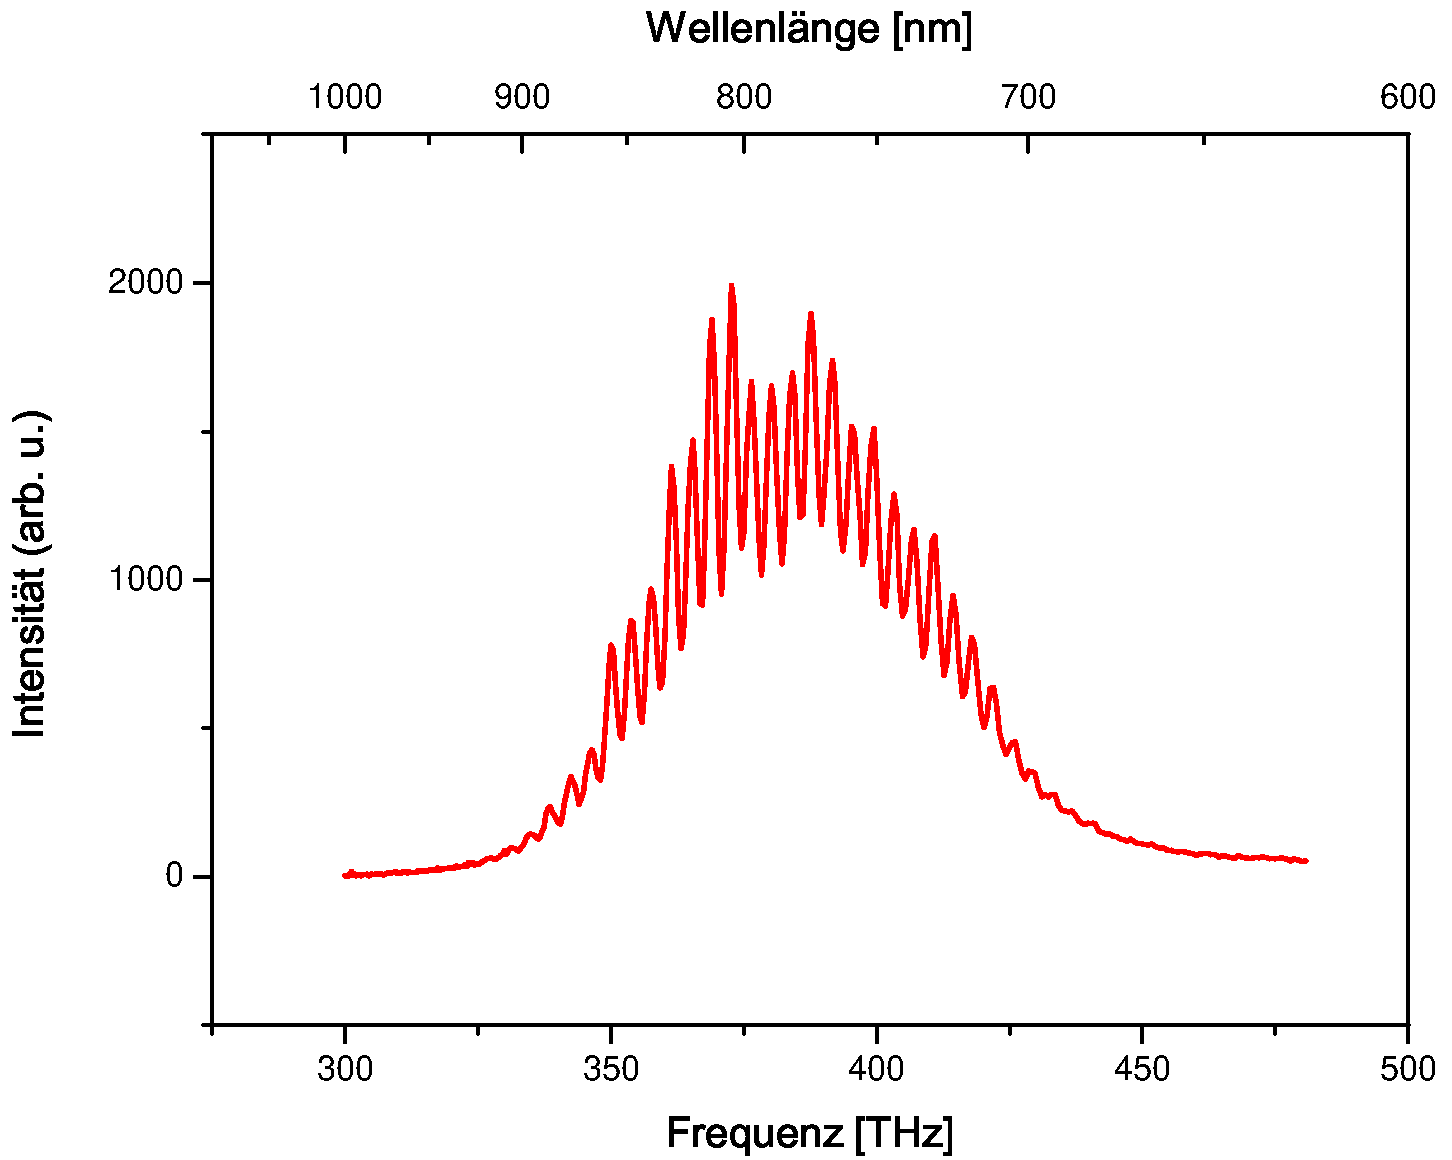
\includegraphics[width=0.49\textwidth]{figures/gratingEtalon}}
   \hfill
   \subfigure[Oszilloskop\label{fig:osziEtalon}]
   {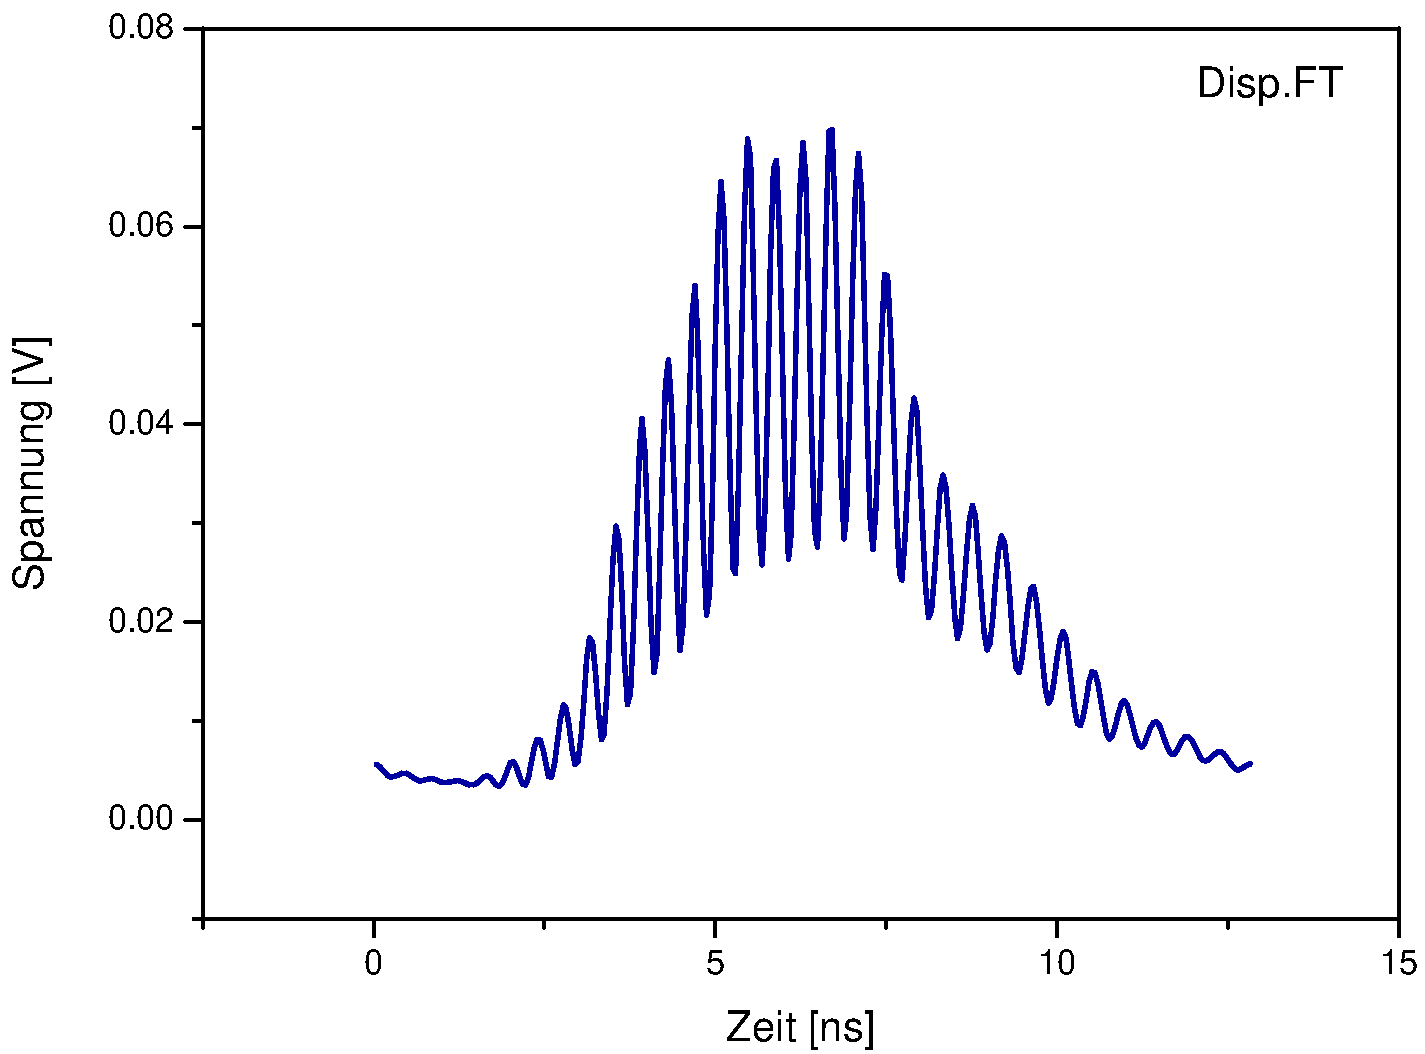
\includegraphics[width=0.49\textwidth]{figures/osziEtalon}}
   \hfill
   \subfigure[Kalibration\label{fig:calibration}]
   {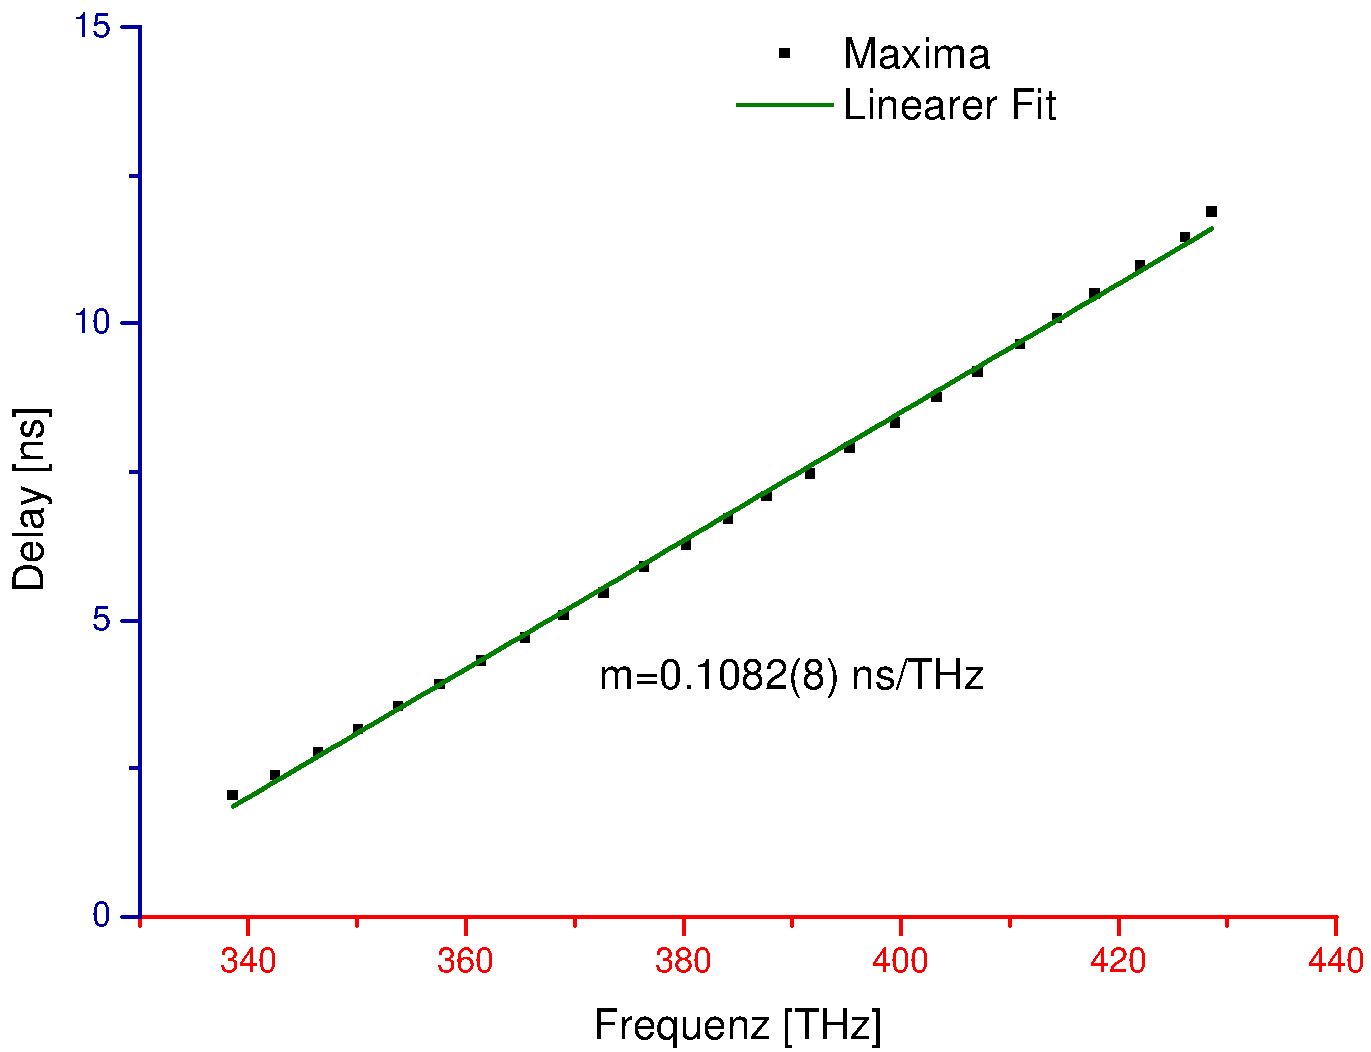
\includegraphics[width=0.7\textwidth]{figures/calibration}}
   \caption{Beschriftung allgemein}
   \label{fig:label-gesamt}
 \end{figure}

\section{Photodiode}
Als nächstes muss noch die Photodiode (Alphalas UPD-40-UVIR-P) charakterisiert werden.
\begin{table}[!htb]
	\centering
	\begin{tabular}{|c|c|}
		\hline
		Risetime & < 40\,ps \\
		Bandbreite & >8.5\,GHz \\
		Spektraler Bereich & 350-1700\,nm \\
		\hline	
	\end{tabular}
\end{table}
Zunächst wird getestet, in welchem Power-Bereich die Photodiode linear reagiert, damit man bei zu künftigen Messungen in diesem Bereich bleibt.
Dies muss für die beiden Modi undispergierter Puls sowie dispergiertes Signal geschehen.
\subsection{Undispergiert}
Man erkennt, dass die Peakamplitude bis ca. 2\,mW linear ansteigt.
Außerdem ist je nach Justage ein Ringing nach dem Puls zu beobachten.

\subsection{Dispergiert}
Bis ca. 10\,mW wächst das Signal linear.
Danach übersteuert man die Photodiode, sodass nicht genug Ladungsträger zwischen zwei Pulsen nachfließen können.

\chapter{Ergebnisse}
Um durch eine langen Messung mit dem Oszilloskop die Entwicklung des Spektrums, etc. darstellen zu können, muss man erst die Pulswiederholrate bestimmen.
Dies geschieht über eine Fouriertransformation des ganzen Signals.
Die Frequenz des höchsten Peaks entspricht der Wiederholrate, das inverse davon also dem Pulsabstand $t_\text{rep}$ bzw. der optischen Cavity-Länge des Lasers.
Da man diese zum Starten ändert, ist die bestimmte Wiederholrate nur für einen kurzen Ausschnitt der Messung korrekt.
Hat man also $t_\text{rep}$ bestimmt, legt man fest, in wie viele äquidistante Punkte man diese Zeit unterteilen möchte.
Dies sollte so gewählt sein, dass die Abstände in etwa zugehörigen Samplingrate entspricht.
Dann interpoliert man die Messdaten an den neuen Zeitpunkten und stellt die Daten anschließend als Matrix dar, trennt also jeden Roundtrip.
Die eine Achse entspricht den Roundtrips, die andere ist die Zeitachse pro Roundtrip.

Zuletzt muss man noch die Änderung der Repetitionsrate bzw. die Abweichung vom richtigen Wert korrigieren.


\section{Doppelpulse 100fs}
\begin{figure}
	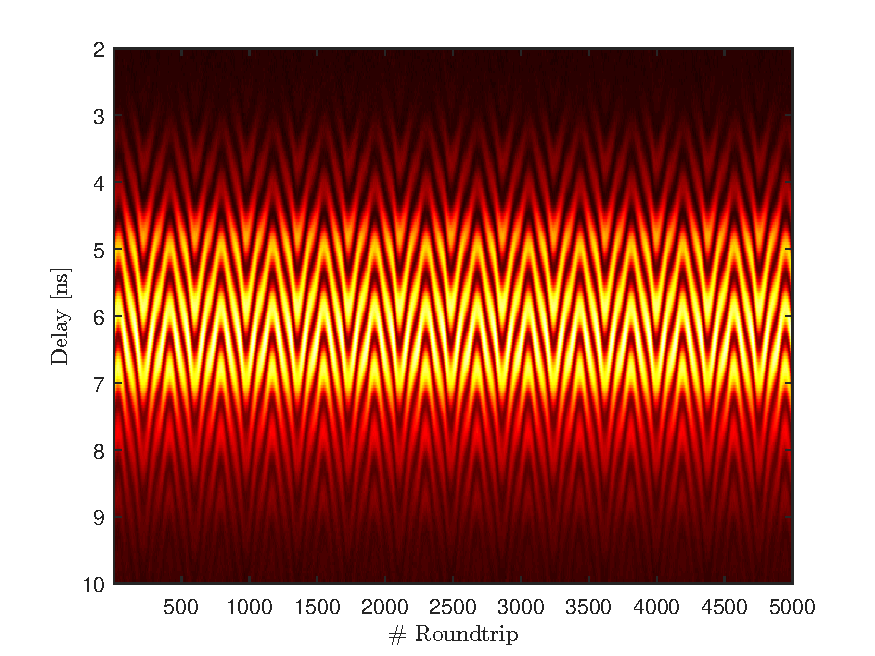
\includegraphics[scale=1.0]{figures/4ms_25GSA_400m_MLrun_runBounceFix_4,58W_Ch_noCB}
\end{figure}

\begin{figure}[!htb]
   \centering
   \subfigure[$P_\text{Pump}=4.58\,$W\label{fig:rBF458}]
   {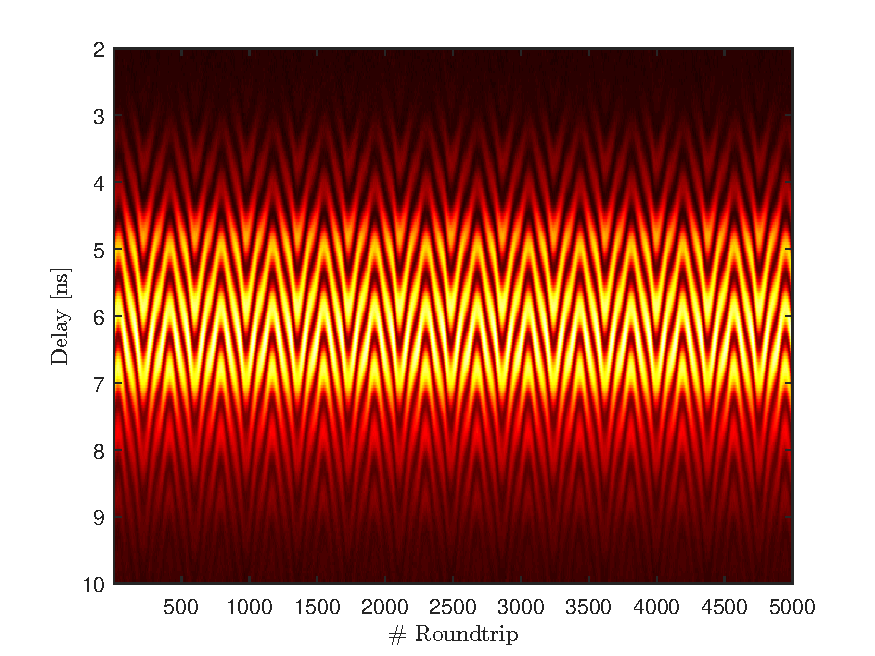
\includegraphics[width=0.49\textwidth]{figures/4ms_25GSA_400m_MLrun_runBounceFix_4,58W_Ch_noCB}}
   \hfill
   \subfigure[$P_\text{Pump}=4.63\,$W\label{fig:rBF463}]
   {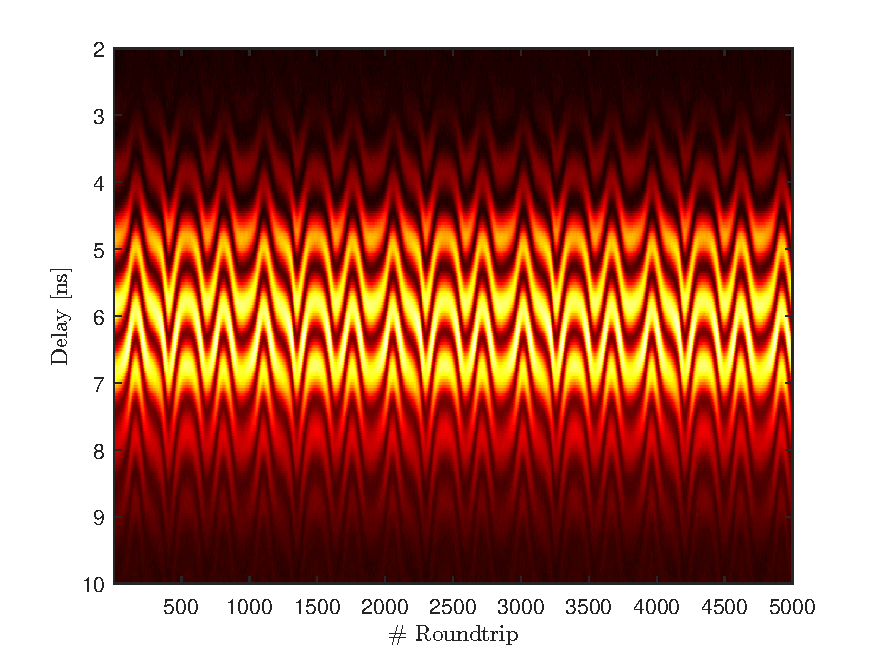
\includegraphics[width=0.49\textwidth]{figures/4ms_25GSA_400m_MLrun_runBounceFix_4,63W_Ch_noCB}}
   \hfill
   \subfigure[$P_\text{Pump}=4.64\,$W\label{fig:rBF464}]
   {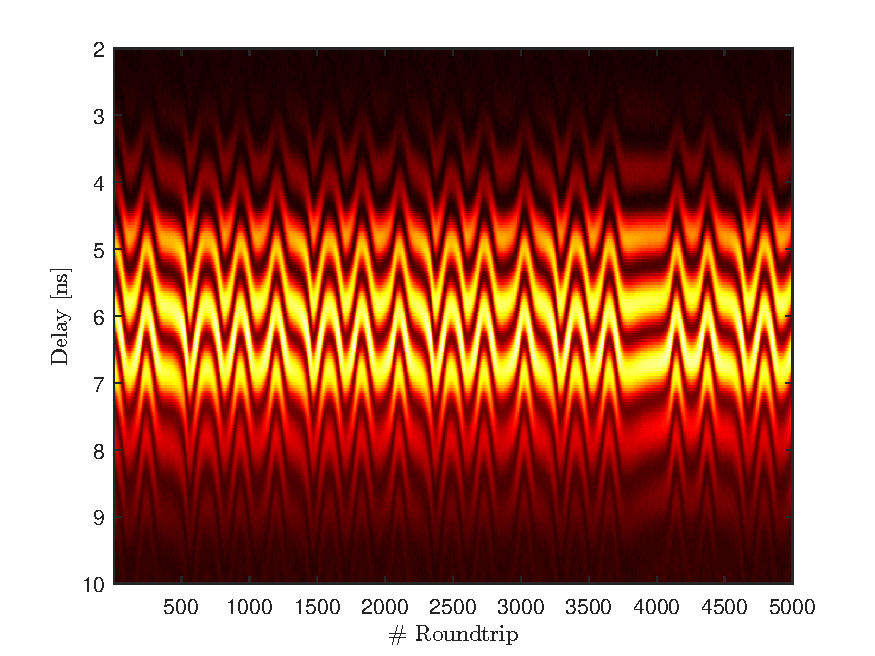
\includegraphics[width=0.49\textwidth]{figures/4ms_25GSA_400m_MLrun_runBounceFix_4,64W_Ch_noCB}}
   \hfill
   \subfigure[$P_\text{Pump}=4.68\,$W\label{fig:rBF468}]
   {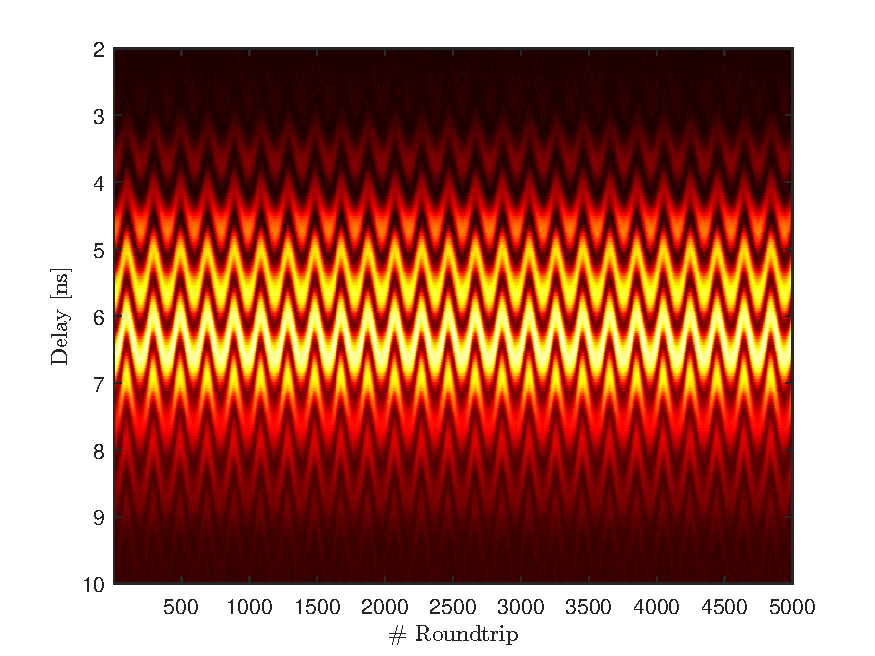
\includegraphics[width=0.49\textwidth]{figures/4ms_25GSA_400m_MLrun_runBounceFix_4,68W_Ch_noCB}}
   \caption{Beschriftung allgemein}
   \label{fig:label-gesamt}
 \end{figure}
 
 \begin{figure}[!htb]
   \centering
   \subfigure[$P_\text{Pump}=4.58\,$W\label{fig:rBF458}]
   {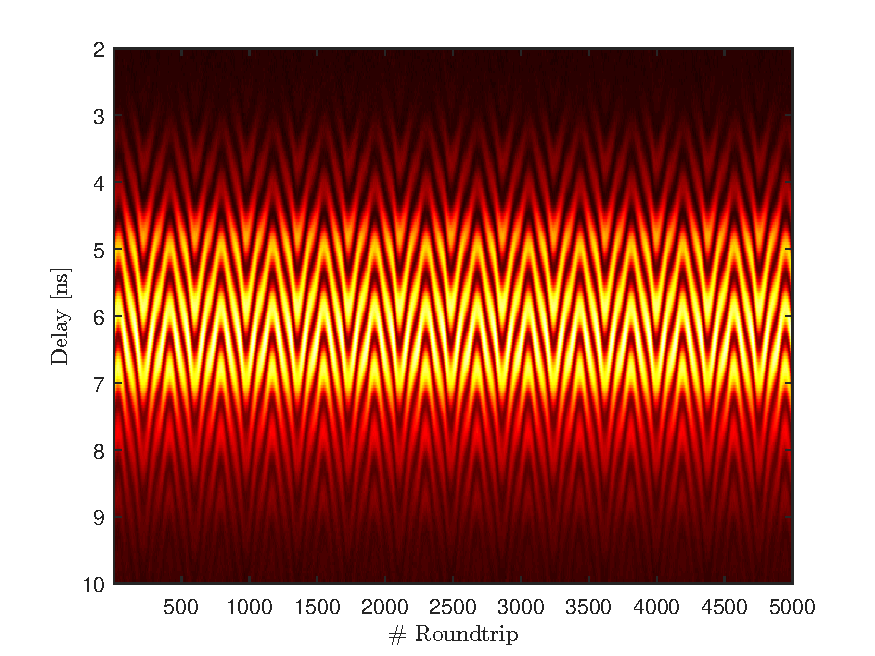
\includegraphics[width=0.6\textwidth]{figures/4ms_25GSA_400m_MLrun_runBounceFix_4,58W_Ch_noCB}}
   \hfill
   \subfigure[$P_\text{Pump}=4.63\,$W\label{fig:rBF463}]
   {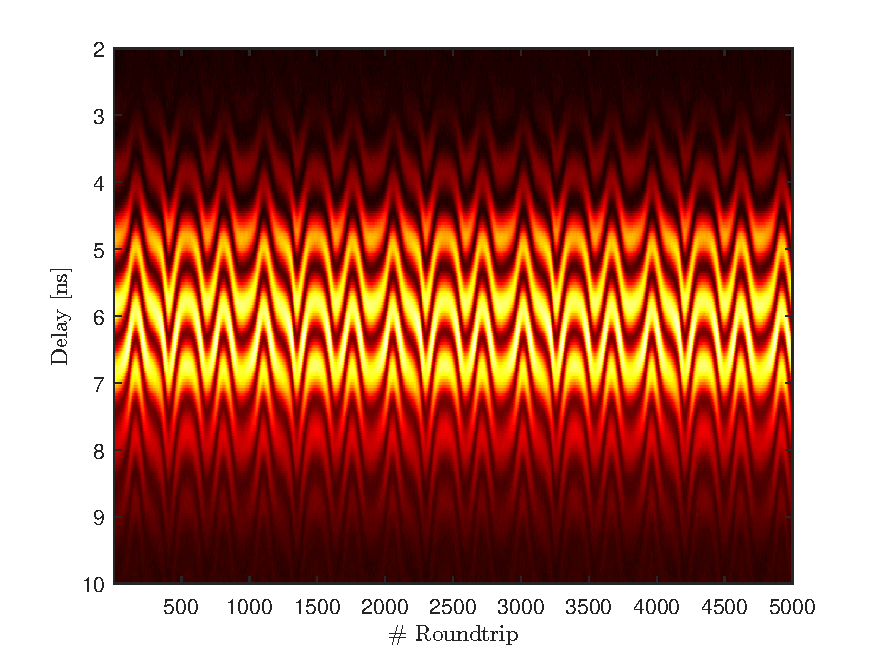
\includegraphics[width=0.6\textwidth]{figures/4ms_25GSA_400m_MLrun_runBounceFix_4,63W_Ch_noCB}}
   \hfill
   \subfigure[$P_\text{Pump}=4.68\,$W\label{fig:rBF468}]
   {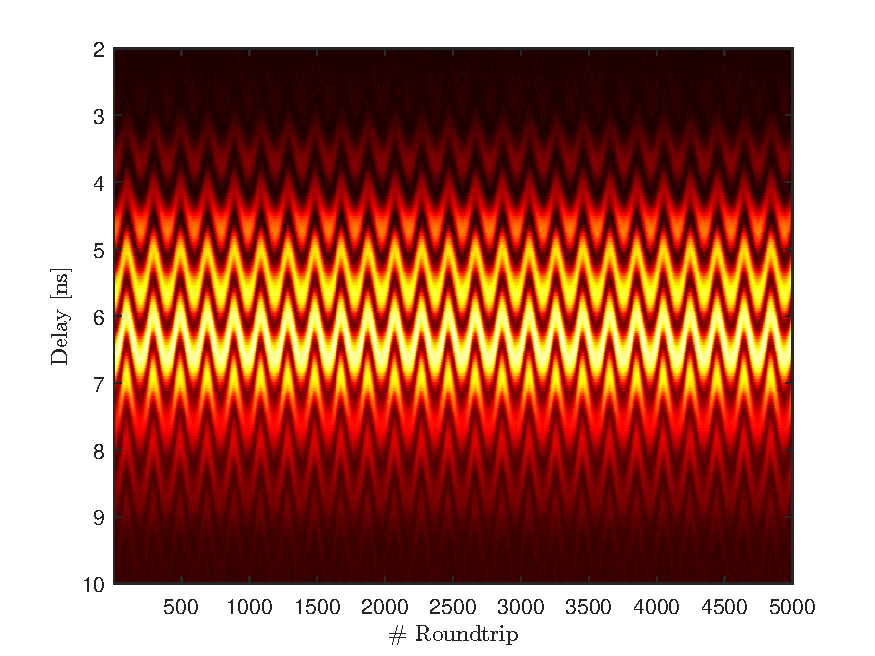
\includegraphics[width=0.6\textwidth]{figures/4ms_25GSA_400m_MLrun_runBounceFix_4,68W_Ch_noCB}}
   \caption{Beschriftung allgemein}
   \label{fig:label-gesamt}
 \end{figure}

\section{Doppelpulse 200fs}

\section{Dreifach-Pulse}

\section{Weiteres}

\chapter{Diskussion}
\section{Colliding Pulse Modelocking}
Während der Messungen konnte das sogennante \textit{Colliding Pulse Modelocking} beobachtet werden.
Dabei laufen zwei Pulse im Laser umher, die sich im Laserkristall treffen und so den Kerr-Effekt beider Pulse sehen, sodass beide eine höhere Verstärkung erfahren.
Dieser Zustand ist sehr stabil und wurde zuerst von \cite{lai_multiple_1997} in einem Ti:Sa-Laser beschrieben.
Interessant ist nun der Prozess bevor dieser stabile Zustand erreicht wird.
Typischerweise modelockt eine Fluktuation, während die anderen Fluktuationen aber nicht völlig aussterben.
Eine weitere Fluktuation wächst nun an, sodass auch diese modelockt.
Daraufhin bewegen sich die beiden Pulse relativ zueinander, da sie nicht gleich stark sind und aufgrund des Kerr-Effektes unterschiedliche optische Weglängen im Laser haben.
Dies geschieht auf einer relativ langen Zeitskala (Größenordnung $~100\,$ms), ist also mit einer normalen Messung (nur 4\,ms) nicht aufzunehmen.
Dazu müsste man in den \textit{FastFrame}-Mode wechseln, kann aber dann nicht jeden Puls aufnehmen.
Außerdem muss man sich bei solch großen Abständen zwischen den Pulsen das undispergierte Signal anschauen.
Die Genauigkeit liegt dort aber nur bei ca. $10\,$ps.

Interessant zu beobachten wäre nun, wie der schwächere Puls das Wandern beendet.
Gleichen sich beide Pulse nur in ihrer Intensität an, dass sie beide genau dann gleich stark sind, wenn sie den perfekten Abstand zueinander haben?
Oder ist eine abklingende Schwingung um diesen zu beobachten?
Wie stabil ist dieser Abstand überhaupt, gibt es auch später noch Oszillationen?

Um all diese Fragen zu beantworten, könnte man den Strahl aufspalten und den einen Teil so verzögern, dass der erste Puls in diesem Arm zeitgleich mit dem zweiten Puls im kürzeren Abschnitt überlappt.
Nun ist die Abstandsinformation auch wieder im Spektrum einkodiert und man kann die Abstände zwischen beiden Pulsen genau messen.


\chapter{Zusammenfassung}
Laser ist komplex, Messmethode ist verdammt cool!

\appendix
\chapter{erster Anhang}
Text\dots
\chapter{zweiter Anhang}
Text\dots

\cleardoublepage
%% Bibliographie. Das Argument muss der Name der BIBTeX-Datenbank stehen.
%% Ein Beispiel fuer eine solche Datenbank finden Sie in bthesis_datenbank.bib
\bibliography{test} 

\chapter*{Danksagung}
Dank\dots

%% Dieser Befehl MUSS am Ende stehen und erzeugt die Erklaerung ueber die
%% benutzten Mittel
\Declaration
\end{document}
